\chapter{Architektur}
\section{siot.net Architektur}
Die Gesamtarchitektur von siot.net mit dem Zusammenspiel mit Android und Android Wear ist auf der Abbildung 7.1 zu betrachten.

Im Zentrum steht das siot.net \gls{IoT}-Center, welches zwingend mit dem siot-Interface (vgl. \cite{siot:cobo}) angesprochen werden muss.

Darunter sind die Sensoren und Aktoren. Diese sind hierarchisch aufgezeigt. Das heisst ein Sensor oder Aktor, von einem Android Wear Gerät, muss die darüber liegenden Stationen durchqueren, um sich am siot.net zu manifestieren. Aus dieser Architektur ist ersichtlich, dass Android Wear Komponenten nicht direkt über ein siot.net Gateway kommunizieren. Dieser Aspekt wird im Abschnitt Netzwerk-Architektur genauer betrachtet.

Am oberen Teil sind die Applikationen eingezeichnet. Diese ziehen nutzten von den Sensoren und Aktoren, welche im siot.net manifestiert sind und Daten senden oder empfangen.
\begin{figure}[h]
  \centering
  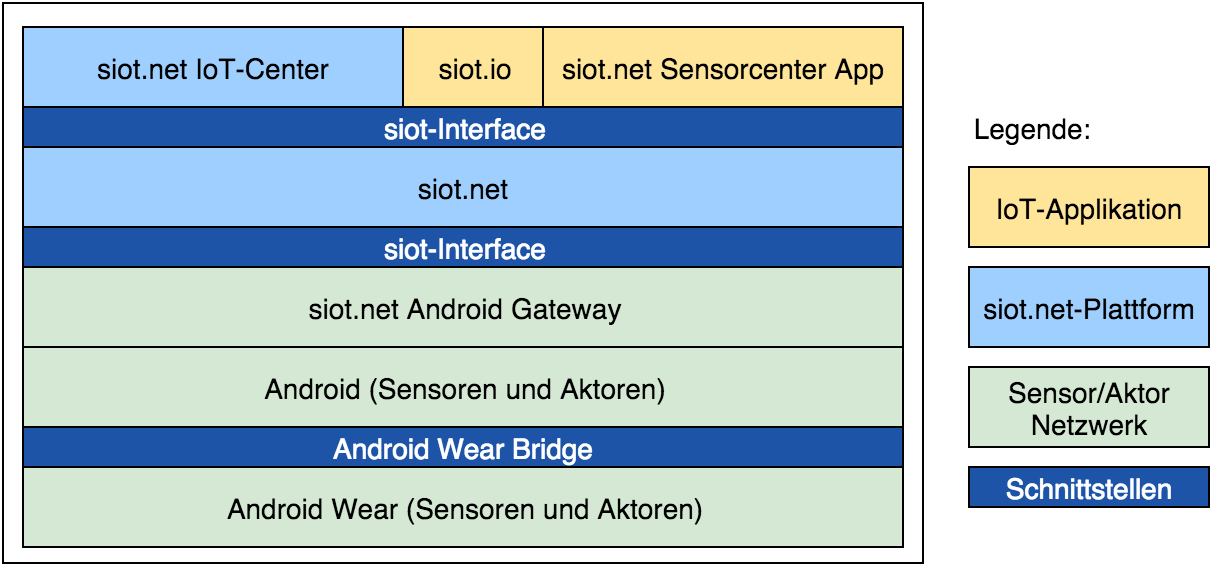
\includegraphics[scale=0.38]{98_Bilder/07_Architektur/ArchitekturSiot}
  \caption[Gesamtarchitektur zu siot.net]{Die Gesamtarchitektur von siot.net im Zusammenspiel mit der Android Welt}
\end{figure}
\newpage
\section{Android Wear Paket Architektur}
Android Wear hat eine strikte Paket Architektur. Abbildung 7.2 veranschaulicht die Übersicht dieser Architektur. Eine Android Wear App muss immer zwingend eine dazugehörige Android App beinhalten. Wenn beide Apps gemeinsam verwendete Klassen haben, müssen diese in ein solches Paket ausgelagert werden. Die in der Android Mobile Paket entwickelten Klassen sollten nicht in einer Android Wear Applikation instanziiert werden. Üblicherweise wird bei der Installation der .apk auf ein Android Smartphone, parallel die Smartwatch App auf die Uhr mit installiert.
\begin{figure}[h]
  \centering
  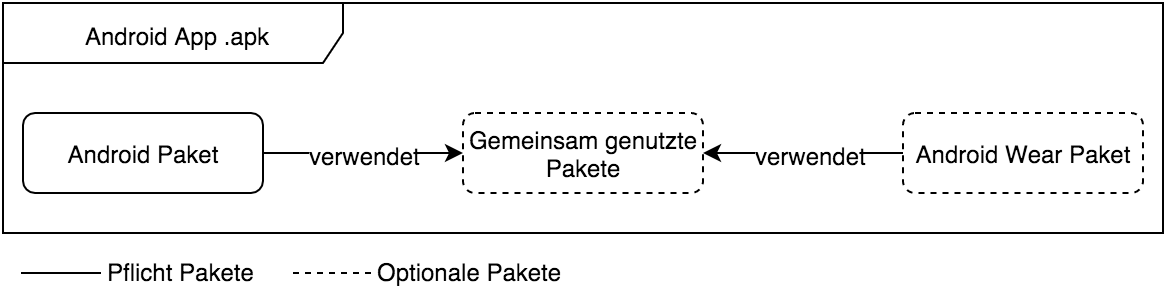
\includegraphics[scale=0.4]{98_Bilder/07_Architektur/AndroidPaketArchitektur}
  \caption[Übersicht Android Wear Paket Architektur]{Übersicht über die einzuhaltende Paketstruktur}
\end{figure}
\section{siot.net Android Applikationsarchitektur}
Die Abbildung 7.3 zeigt die Softwarearchitektur, welche für Android und Android Wear Applikationen im siot.net Umfeld spezifiziert wurde. Mobile und Wearable Apps für siot.net können so am effizientesten konzipiert werden.
\begin{figure}[h]
  \centering
  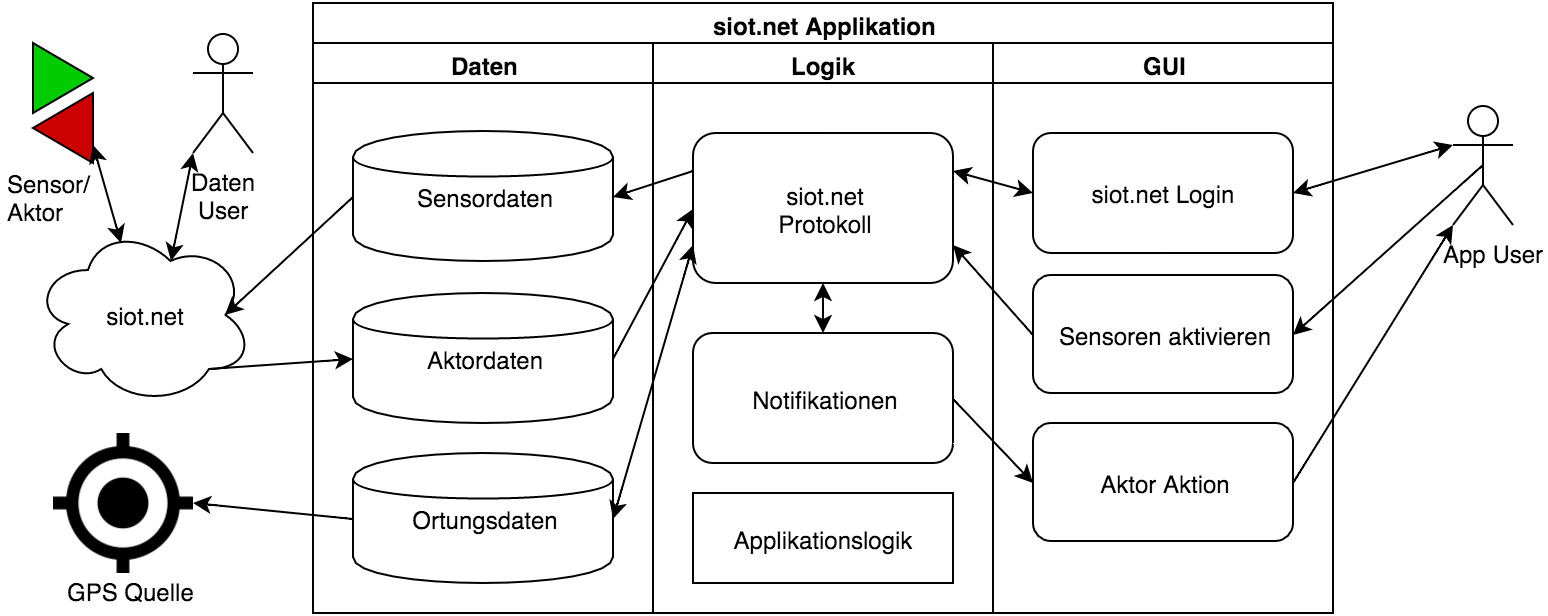
\includegraphics[scale=0.3]{98_Bilder/07_Architektur/siotAppArchitektur}
  \caption[Übersicht siot.net Applikationsarchitektur]{Applikationsarchitektur für siot.net Anwendungen}
\end{figure}
\newpage
\section{Netzwerk-Architektur}
\subsection{geplante Architektur}
\begin{figure}[h]
  \centering
  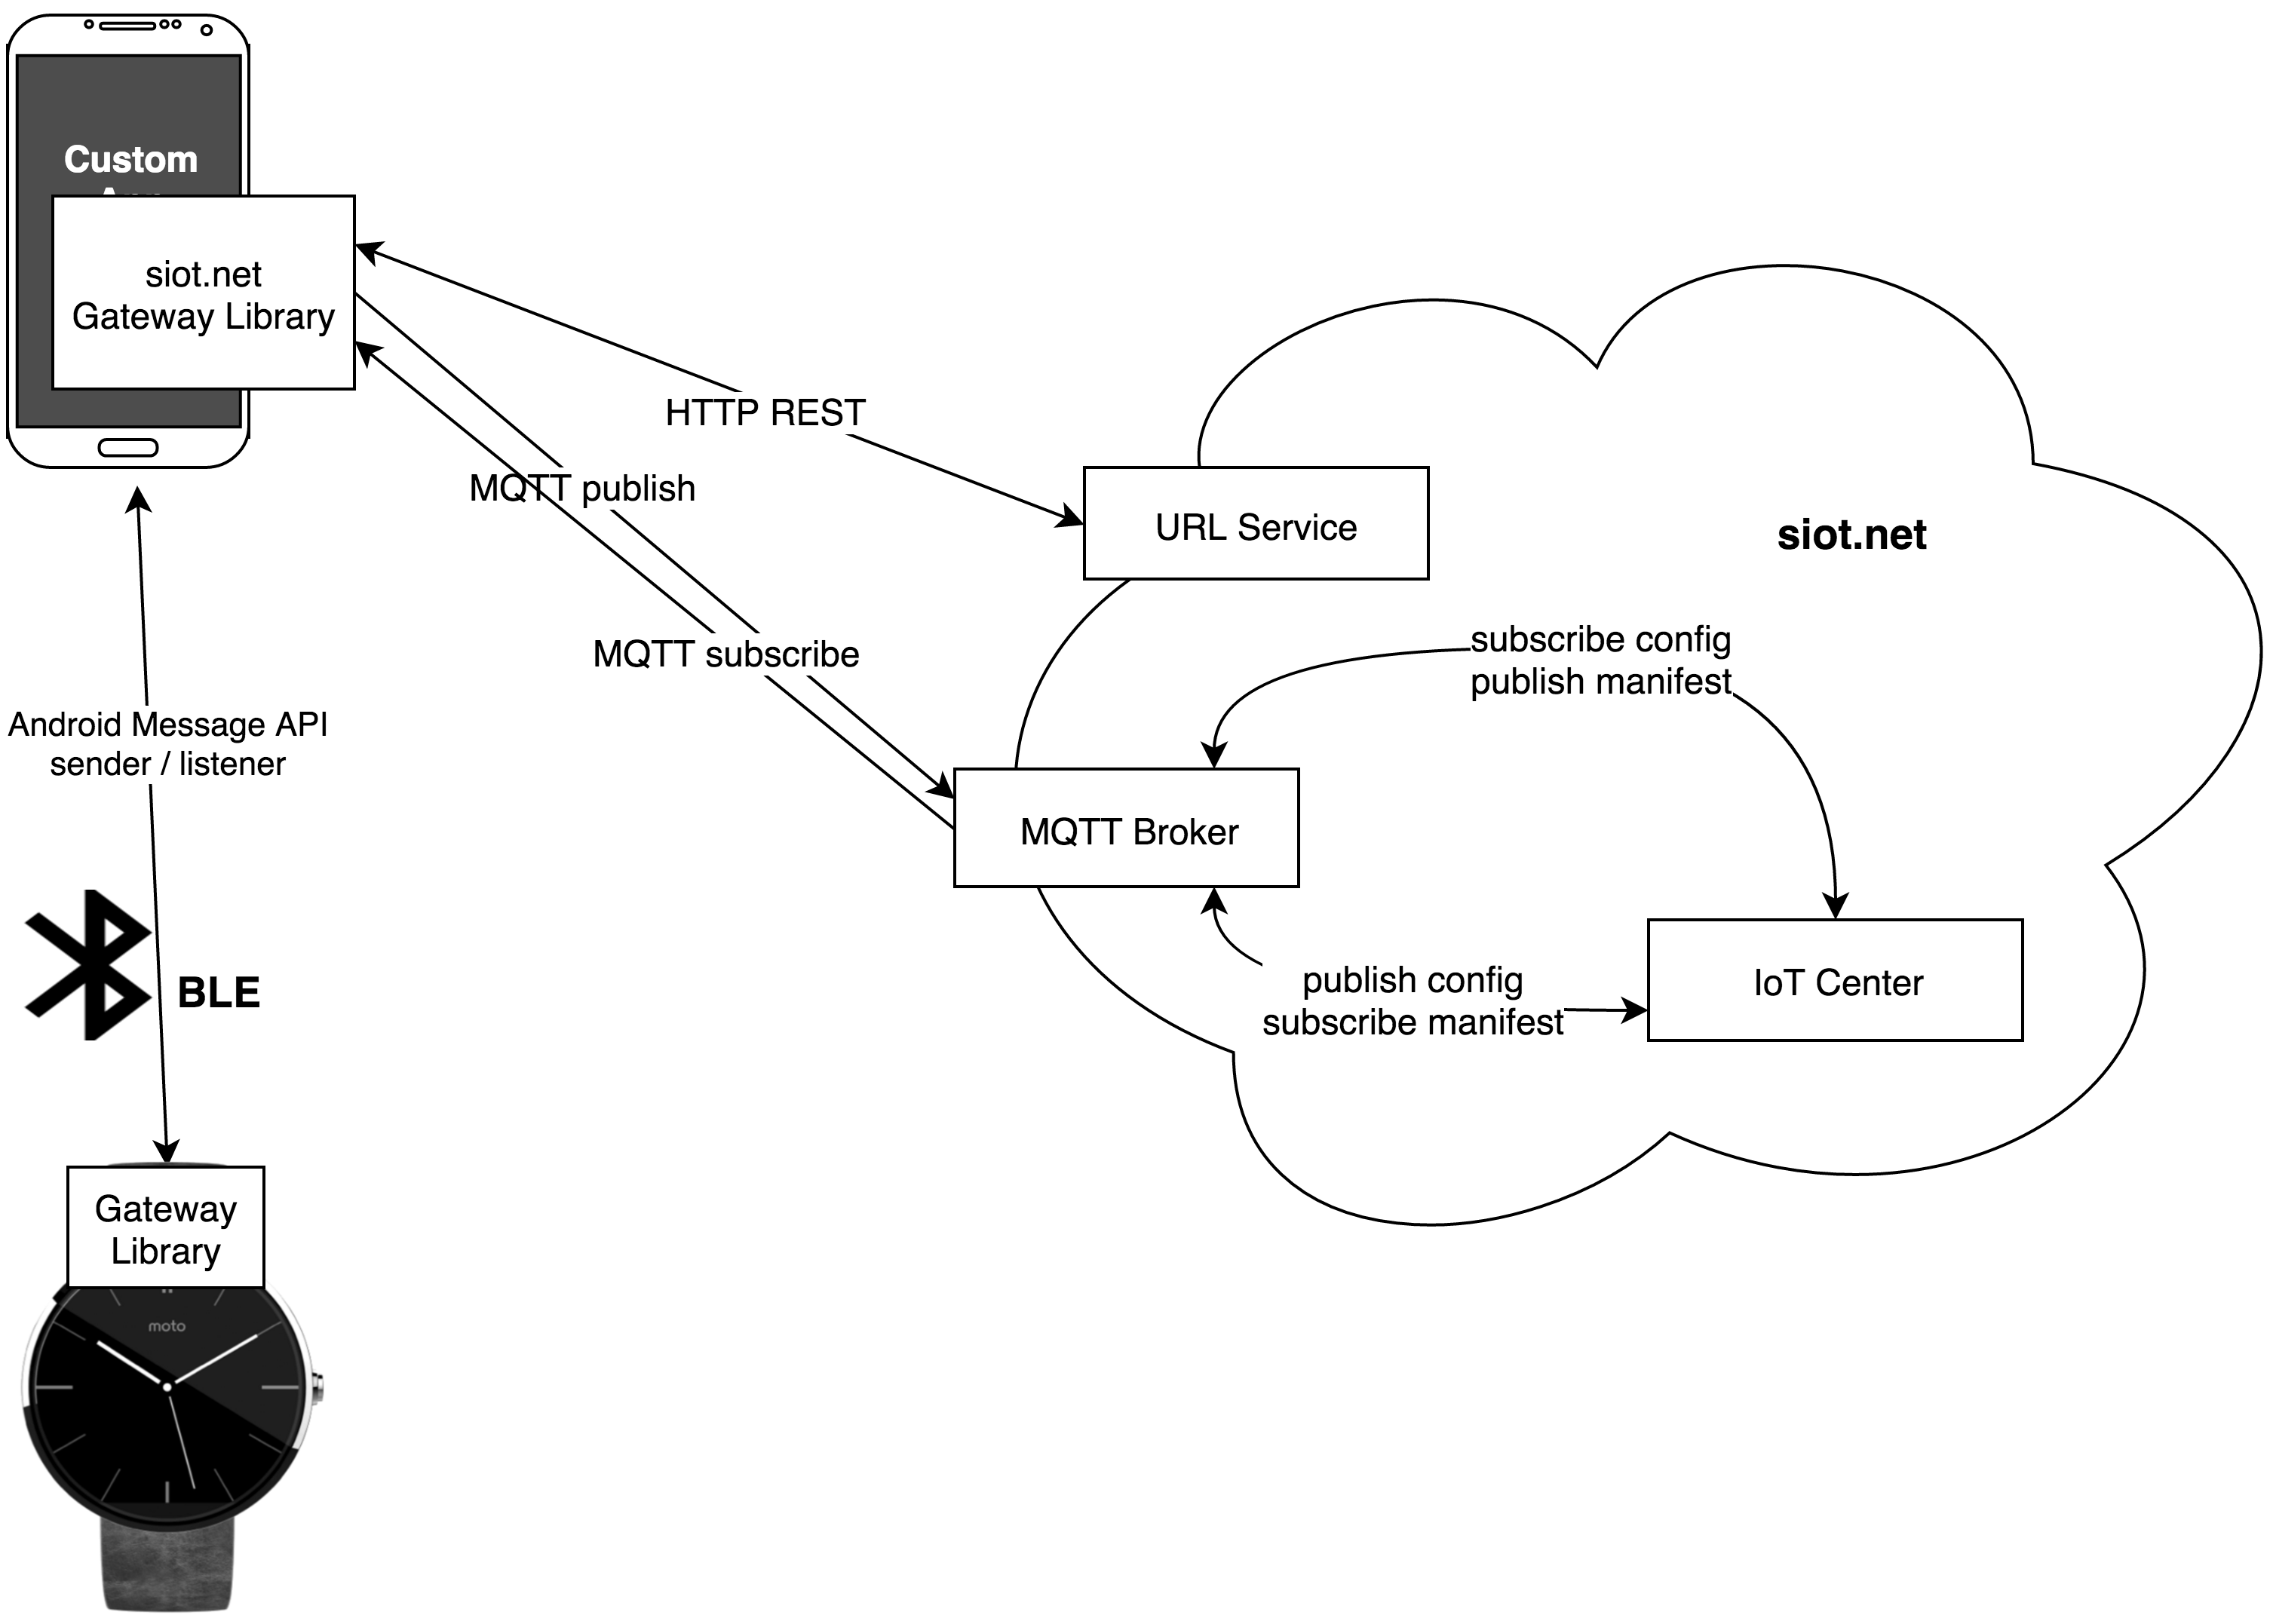
\includegraphics[scale=0.15]{98_Bilder/07_Architektur/01_Architektur}
  \caption[Geplante Netzwerk-Architektur mit \gls{URL}/ohne WLAN]{Geplante Kommunikation zwischen Smartwatch und Smartphone, sowie Smartphone und siot.net}
\end{figure}
Die Abbildung 7.4 visualisiert, wie die Kommunikation zwischen der Smartwatch, dem Smartphone und der siot.net-Plattform stattfinden soll. Im Falle, dass die Smartwatch eine Bluetooth Low Energy (\gls{BLE}) Verbindung mit dem Smartphone aufweist, wird das Smartphone via \gls{REST} und \gls{MQTT} mit der siot.net-Plattform Daten austauschen. Dabei dient das Mobiltelefon als das Gateway von der Smartwatch zur \gls{IoT}-Cloud. Die Android Wear Uhr versendet die Daten, per Android Message\gls{API} via \gls{BLE} zum Android Smartphone. Dies leitet die Pakete mit Hilfe des \gls{MQTT} Protokoll weiter ans siot.net. Diese Variante der Datenübermittlung ist sehr viel stromsparender, als jene die in Abbildung 7.5 aufgezeigt wird.\\
Das Bridging muss in der Smartphone Begleit-App (Android Paket) der Smartwatch Applikation (Android Wear Paket) implementiert sein.
\newpage
\begin{figure}[h]
  \centering
  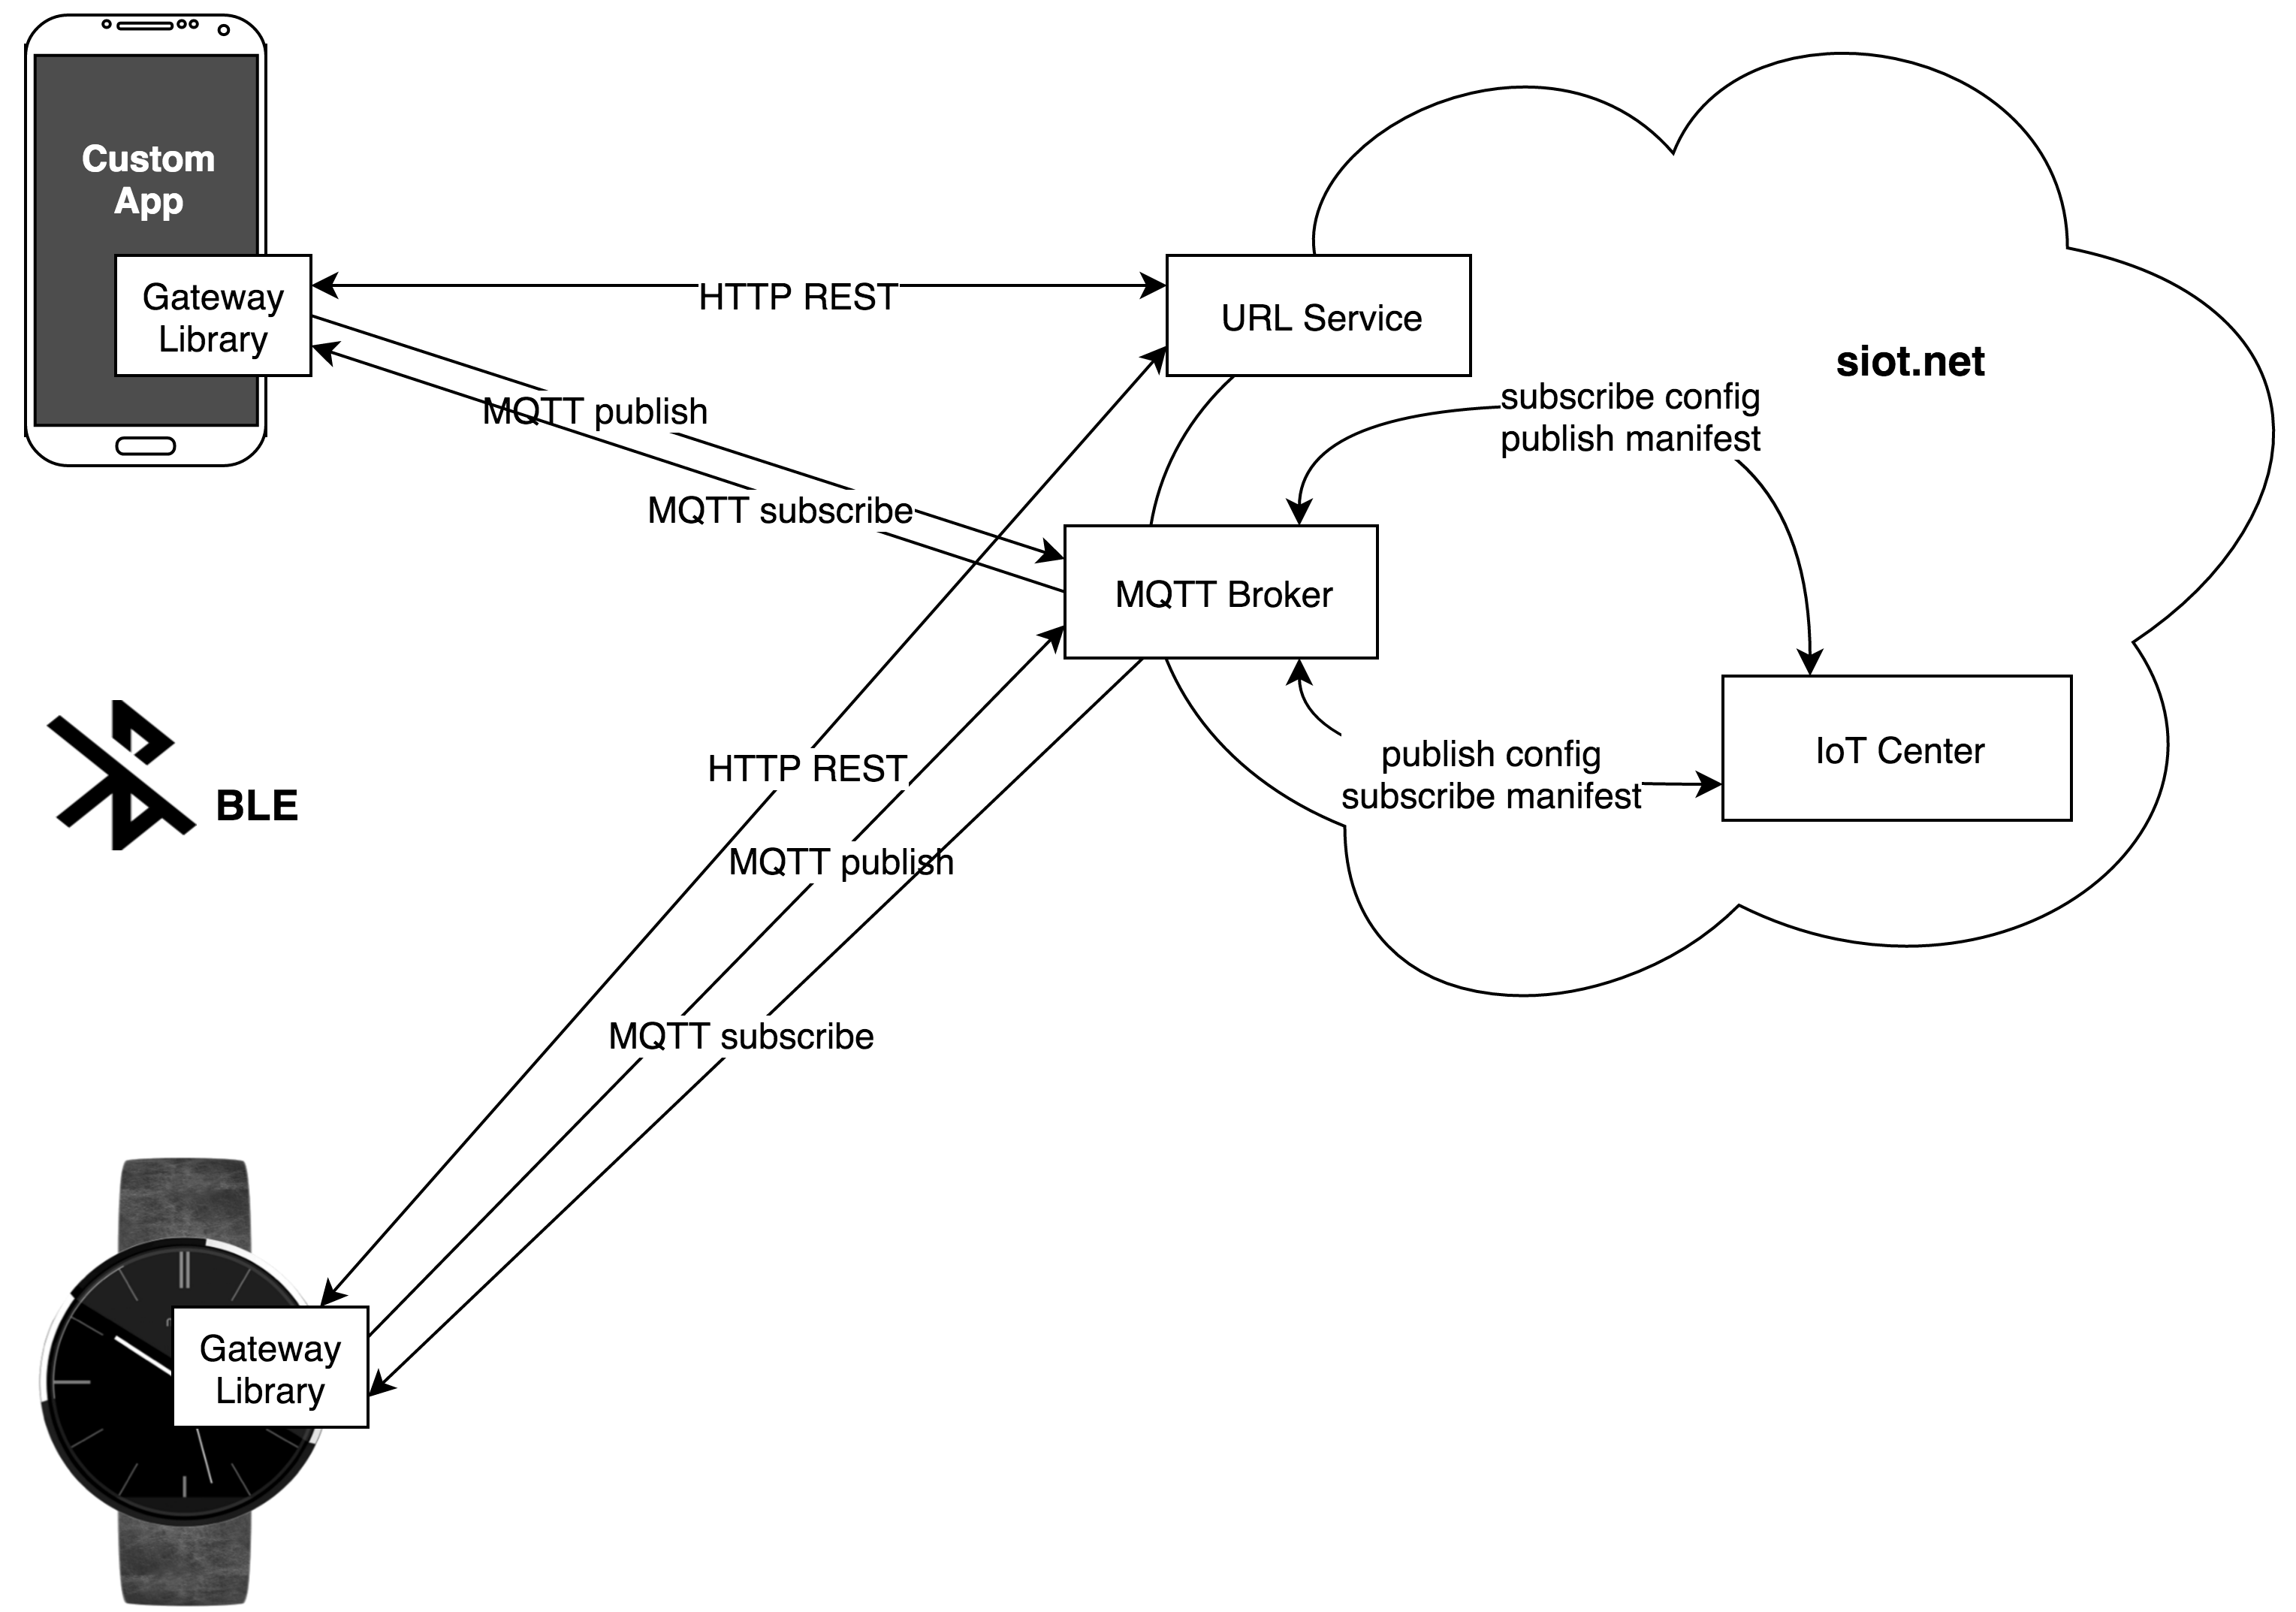
\includegraphics[scale=0.15]{98_Bilder/07_Architektur/02_Architektur}
  \caption[Geplante Netzwerk-Architektur ohne BLE/mit WLAN]{Geplante Kommunikation zwischen Smartwatch und siot.net, sowie Smartphone und siot.net}
\end{figure}
Bei Abbruch der Verbindung von Smartwatch zu Smartphone, soll die Computeruhr die Kommunikation zum siot.net selber übernehmen. Dazu muss zuerst über \gls{REST} die URL des \gls{MQTT} Broker ermittelt werden, um folglich eine Kopplung durchzuführen. Diese Architektur ist auf Abbildung 7.5 zu betrachten. Weil die Android Smartwatches keine direkte Internetverbindung zulassen, kann diese gewünschte Architektur noch nicht umgesetzt werden. Wenn diese Beschränkung durch das Betriebssystem aufgelöst wird, wäre die Architektur bereits spezifiziert.

\newpage
\subsection{effektive Architektur}
\begin{figure}[h]
  \centering
  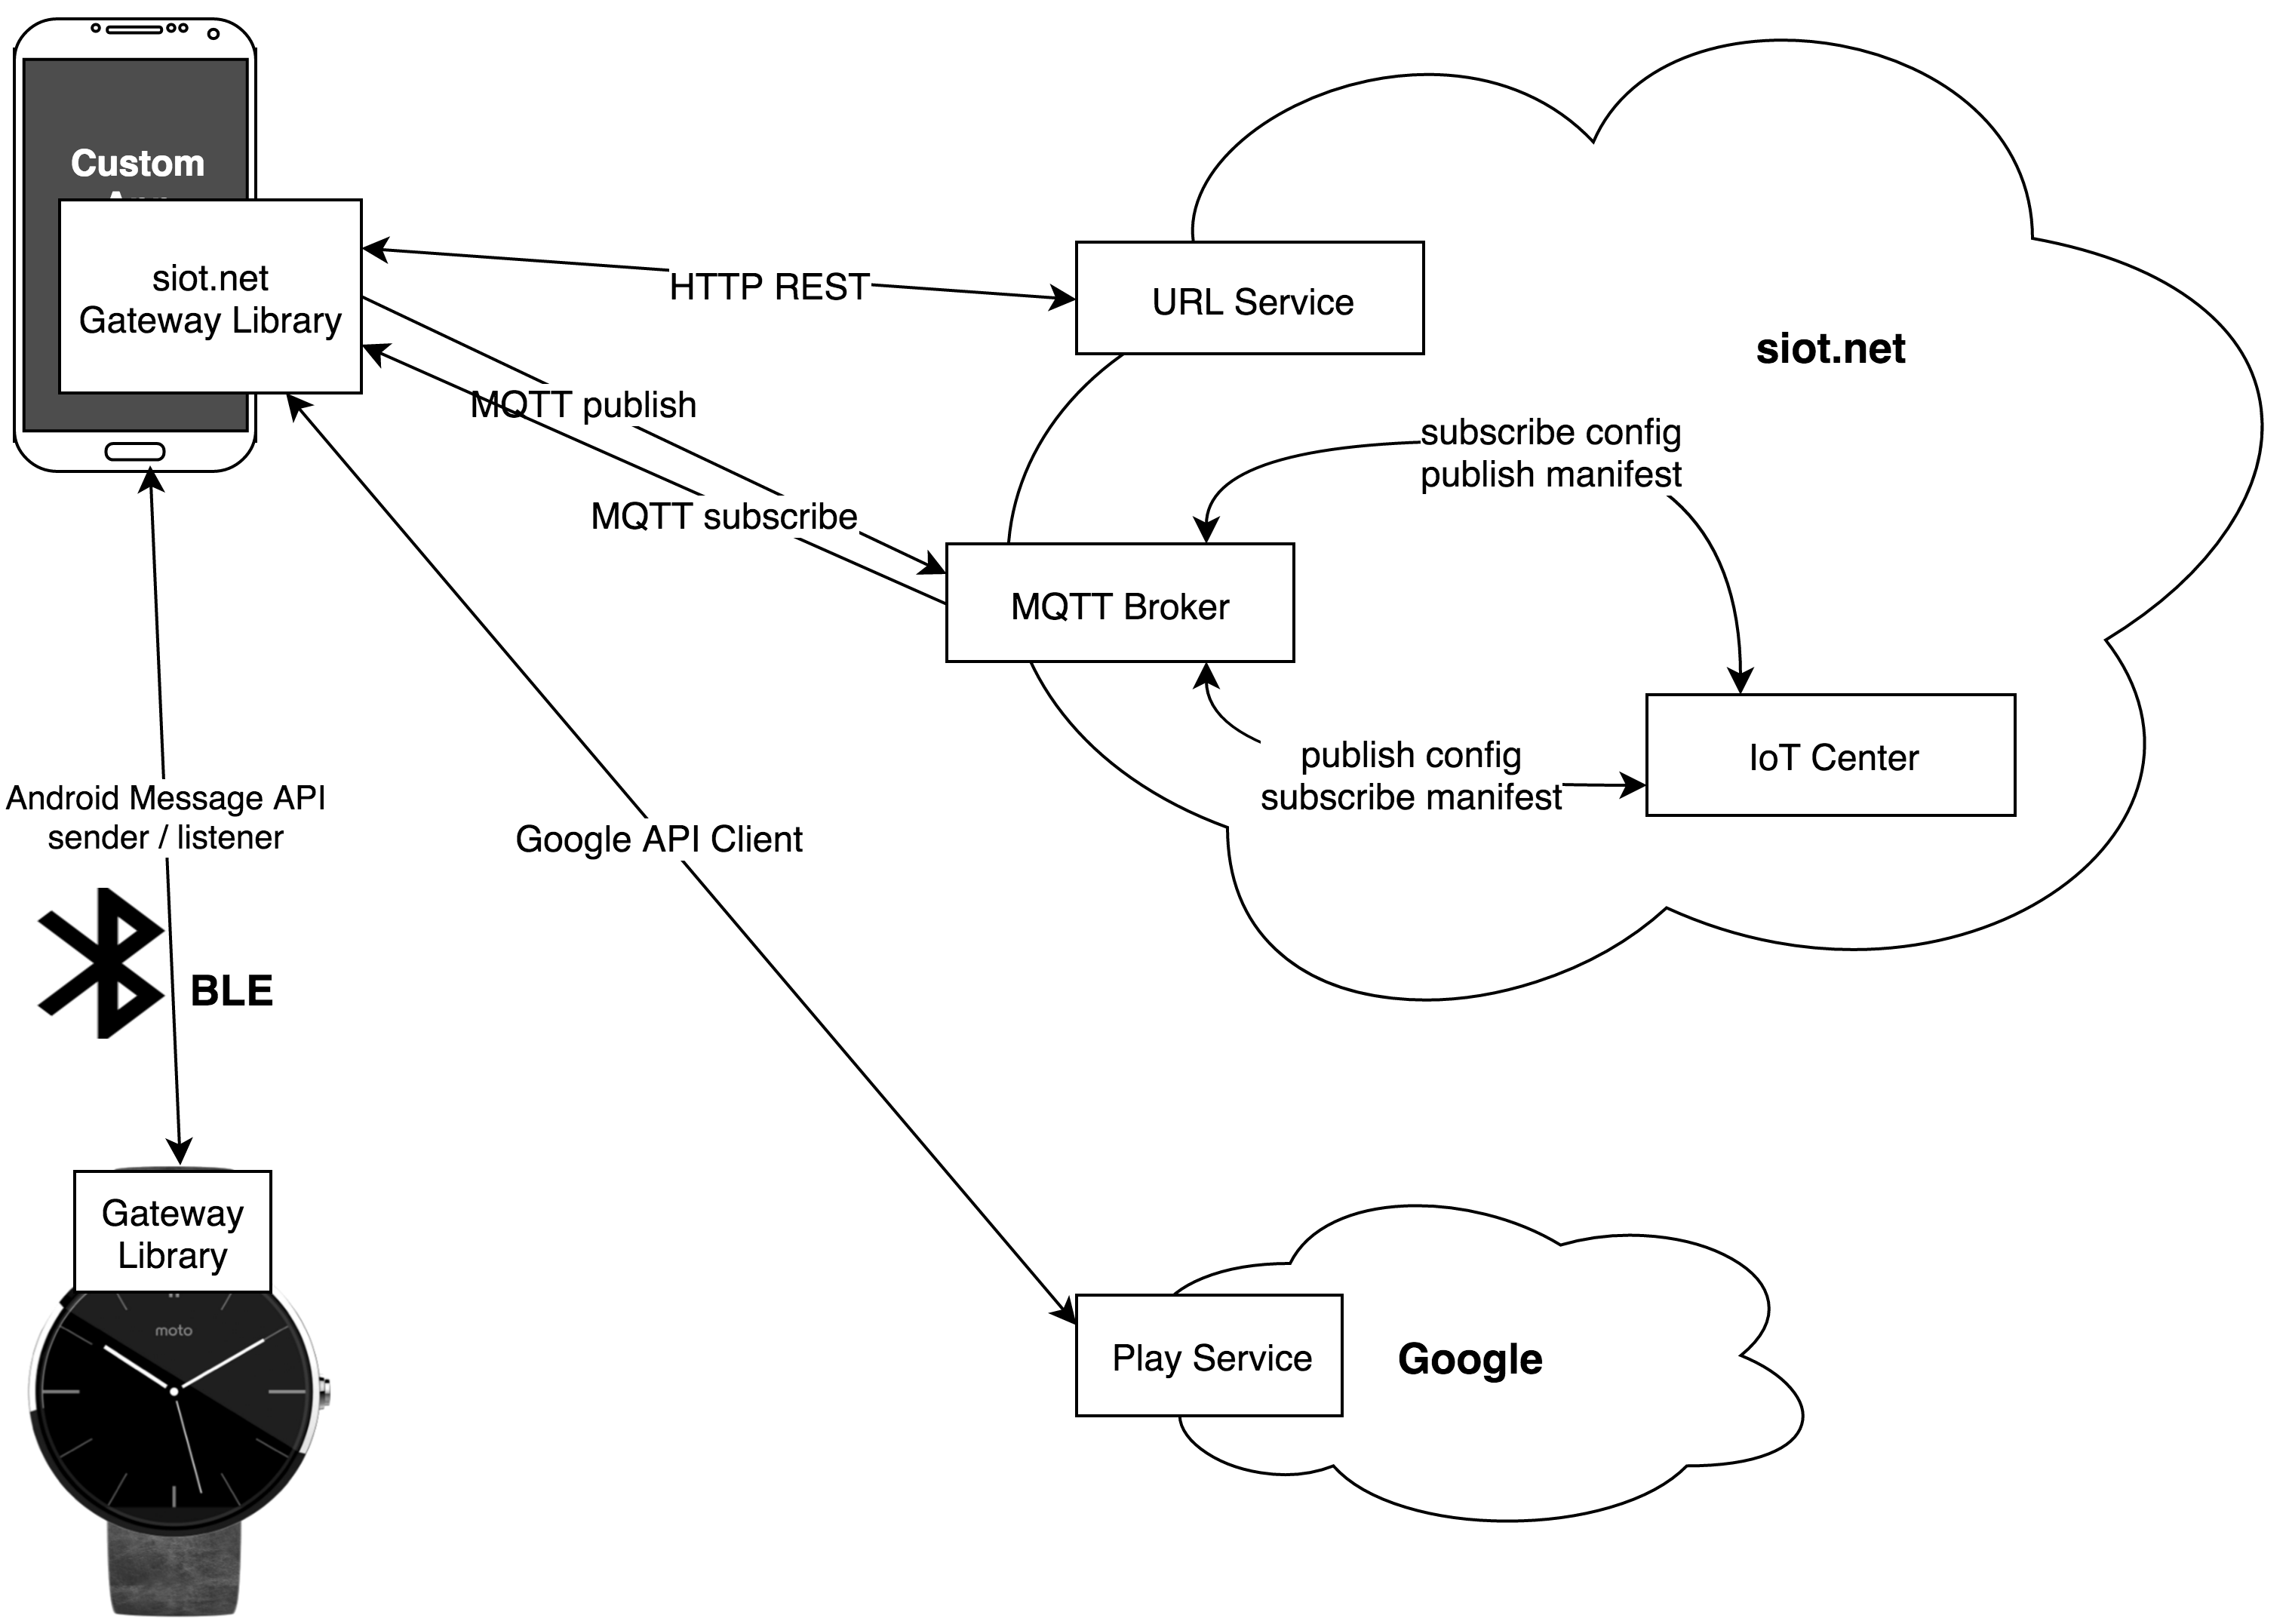
\includegraphics[scale=0.15]{98_Bilder/07_Architektur/03_Architektur}
  \caption[Effektive Netzwerk-Architektur mit BLE/ohne WLAN]{Effektive Kommunikation zwischen Smartwatch und siot.net, sowie Smartphone und siot.net}
\end{figure}
Diese Architektur (siehe Abbildung 7.6) unterscheidet sich geringfügig zu jener auf Abbildung 7.4. Hier kommt nun die Google Cloud dazu. Diese Anbindung ist notwendig, da Android für die Kommunikation über die Android Message\gls{API} eine eindeutige Identität verlangt. Es muss vorhergehend eine NodeId über den Google Play Service eingefordert werden. Dank dieser NodeId dürfen die Geräte (Smartphone und Smartwatch benötigen jeweils eine eindeutige Identifikation) mittels Message\gls{API} Nachrichten transferieren. Der Datenaustausch geschieht dann direkt via \gls{BLE}. Diese Netzwerk-Architektur kommt zum tragen, wenn die Kopplung von Smartwatch und Smartphone über Bluetooth Smart steht.

\newpage
\begin{figure}[h]
  \centering
  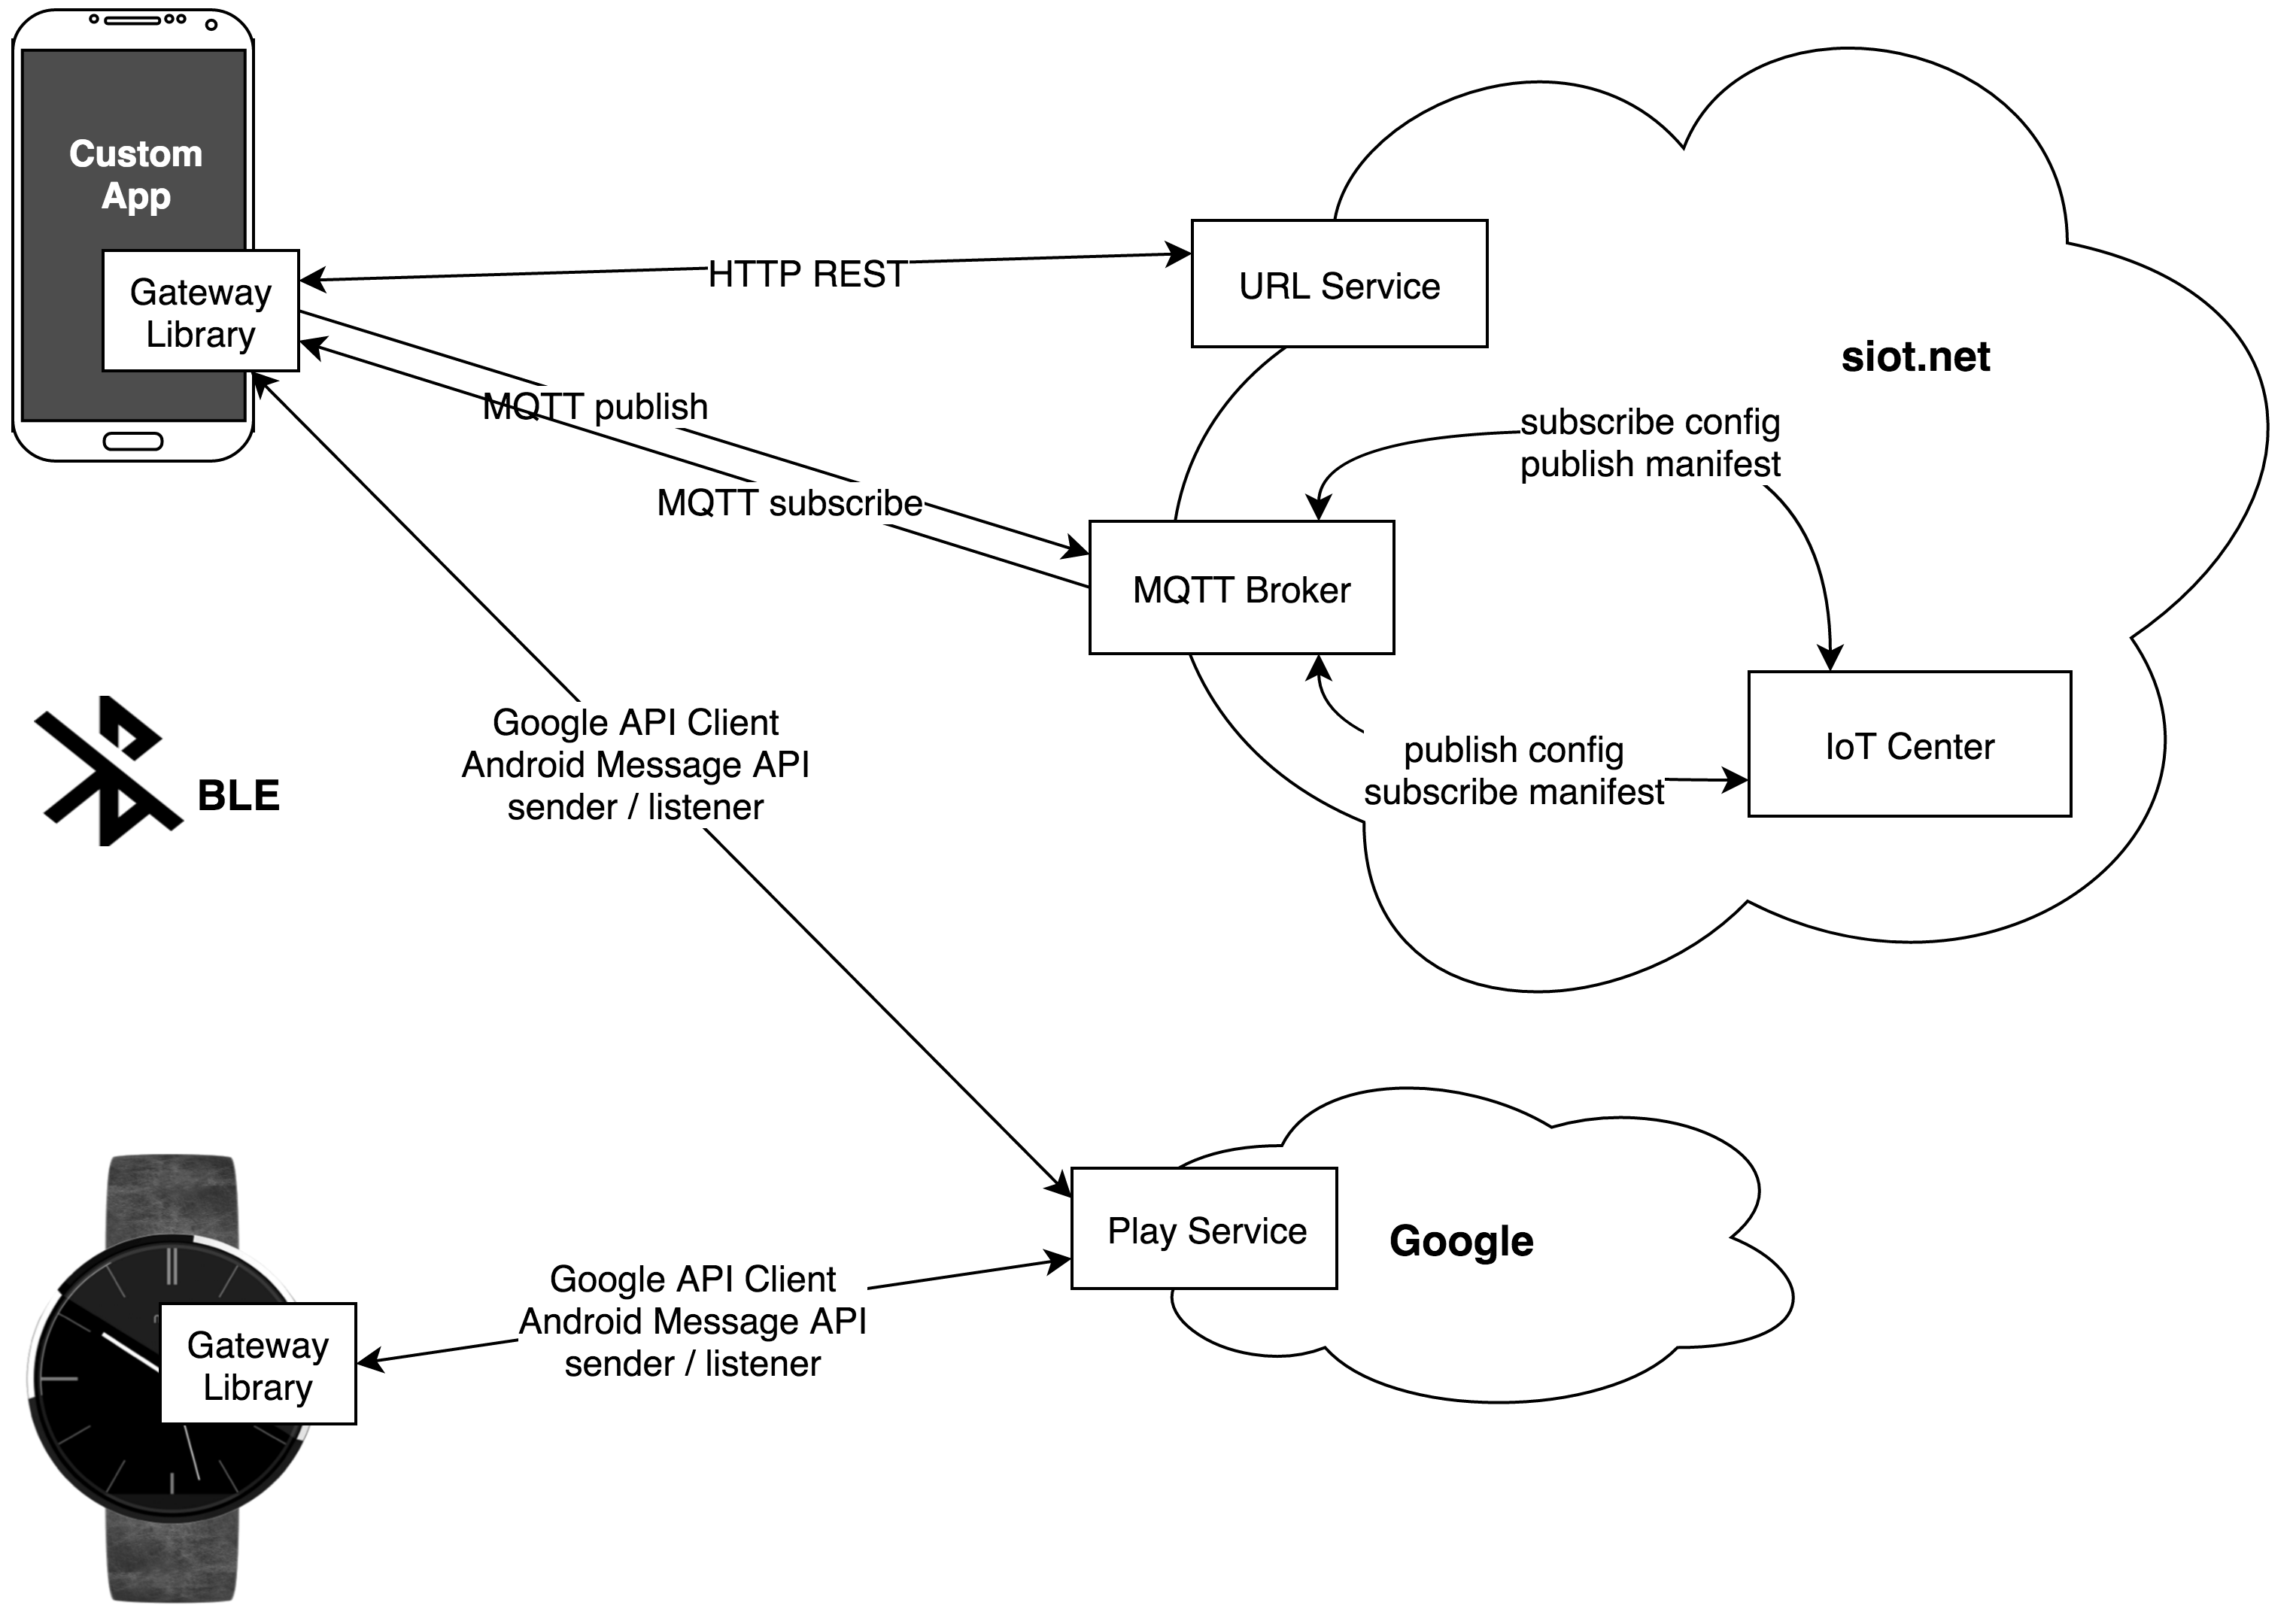
\includegraphics[scale=0.15]{98_Bilder/07_Architektur/04_Architektur}
  \caption[Effektive Netzwerk-Architektur ohne BLE/mit WLAN]{Effektive Kommunikation zwischen Smartwatch und siot.net, sowie Smartphone und siot.net}
\end{figure}
Abbildung 7.7 zeigt die funktionierende Architektur, wenn keine intakte \gls{BLE} Verbindung vorhanden ist. Diese differenziert sich wesentlich von der geplanten Netzwerk-Definition. Auch hier spielt der Faktor Android eine grosse Rolle. Es verbietet Android Wear Geräten den direkten Kontakt zum Internet. So ist hier eine Verbindung über den Google Play Service zum Smartphone nötig. Bei dieser Anbindungsart werden die Daten via Google Cloud an das Android Handy gesendet. Dieses muss dann in jedem Fall als siot.net Gateway fungieren.\\
Der grosse Nachteil dieser Variante ist, dass die Smartwatch nicht als autonomes Gerät fungieren kann. Wenn das Smartphone nicht erreichbar ist, z.B. Akku leer oder keine Netzwerkverbindung, ist die Computeruhr für siot.net nutzlos.
